% RESULTADOS-------------------------------------------------------------------

\chapter{RESULTADOS}
\label{chap:resultados}

%Cada capítulo deve conter uma pequena introdução (tipicamente, um ou dois parágrafos) que deve deixar claro o objetivo e o que será discutido no capítulo, bem como a organização do capítulo. 

\section{Análise modal numérica}
\label{sec:resultmodal}

Na análise modal, as frequências naturais obtidas para os dois casos mantiveram-se afastadas da faixa de operação da turbina. Considerando uma TSR entre 2 e 3,5 e uma faixa de velocidade comumente encontrada entre 1 e 2 $m/s$ tem-se uma faixa de frequências de operação variando entre 0,62 e 2,16 $Hz$ que se encontra distante das frequências naturais encontradas para os casos analisados conforme apresentado na \autoref{tab:resultfreqturbina}. Tal verificação vem confirmar a possibilidade de utilização da consideração de 1 GDL. 

\begin{table}[h]
	\centering
	\caption{Frequências naturais obtidas [Hz].}
	\label{tab:resultfreqturbina}	
	    \begin{tabular}{c c c}
        \hline Modo &  &  \\
         & Maciço & Tubo \\
        \hline        
		1 & 9,04 & 7,54 \\
		2 & 9,08 & 7,55 \\
		3 & 13,40 & 9,80 \\
		4 & 28,68 & 20,19\\
		5 & 28,74 & 20,21 \\
		6 & 30,32 & 24,56 \\
		\hline
    \end{tabular}

	\fonte{Autoria própria.}
\end{table}

As \autoref{fig:resultmodomacico} e \autoref{fig:resultmodotubos} apresentam algumas respostas esperadas para o primeiro e sexto modo de vibração. Nelas é possível verificar a importância da verificação das frequências de operação da turbina, que caso negligenciado pode levar a sérios danos. Também pode-se verificar que a utilização do tubo em comparação aos eixos maciços levaram a maiores deformações.    

\begin{figure}	
	\caption{Modos de vibração do sistema com eixo e braço maciços.}
	\label{fig:resultmodomacico}
	\begin{subfigure}{0.5\textwidth}
		\centering
		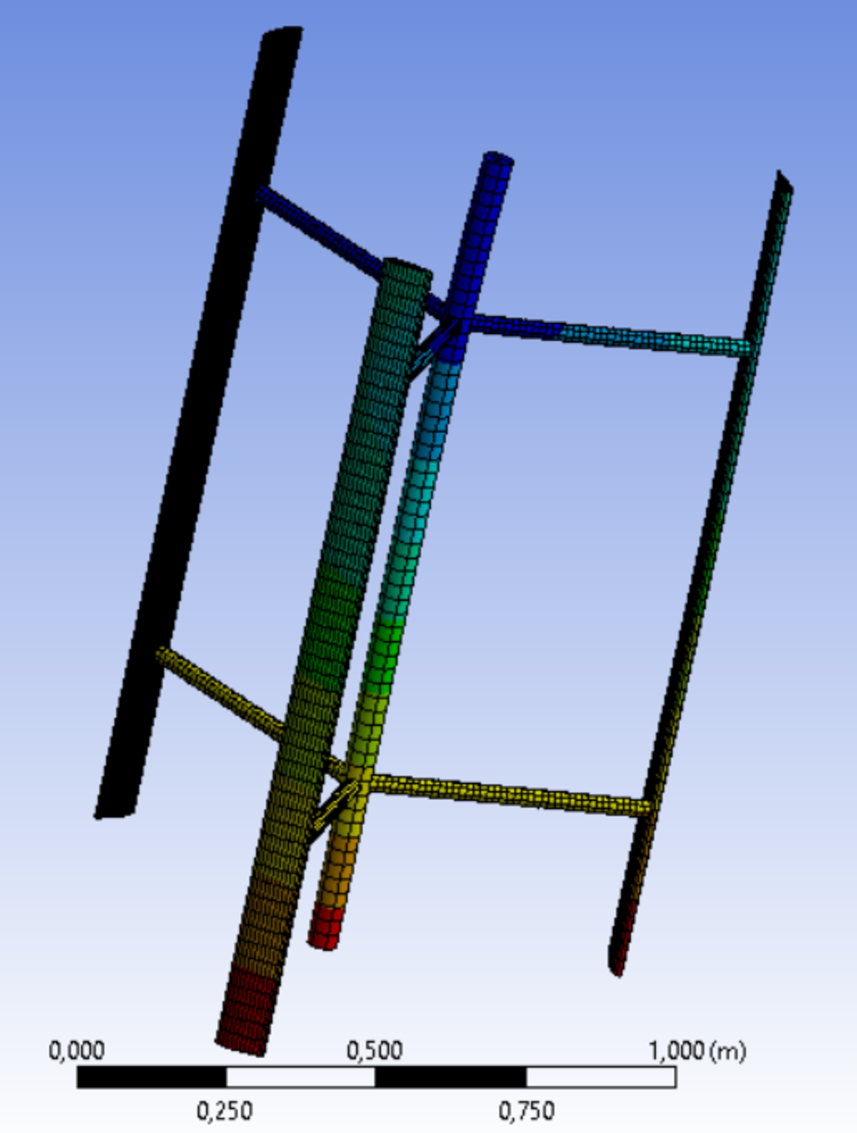
\includegraphics[width=1.0\textwidth]{figuras/resultmodalmacico1.pdf}
		\caption{Primeiro modo.}
		\label{subfig:resultmodomacicomodo1}
	\end{subfigure}
	\begin{subfigure}{0.5\textwidth}
		\centering
		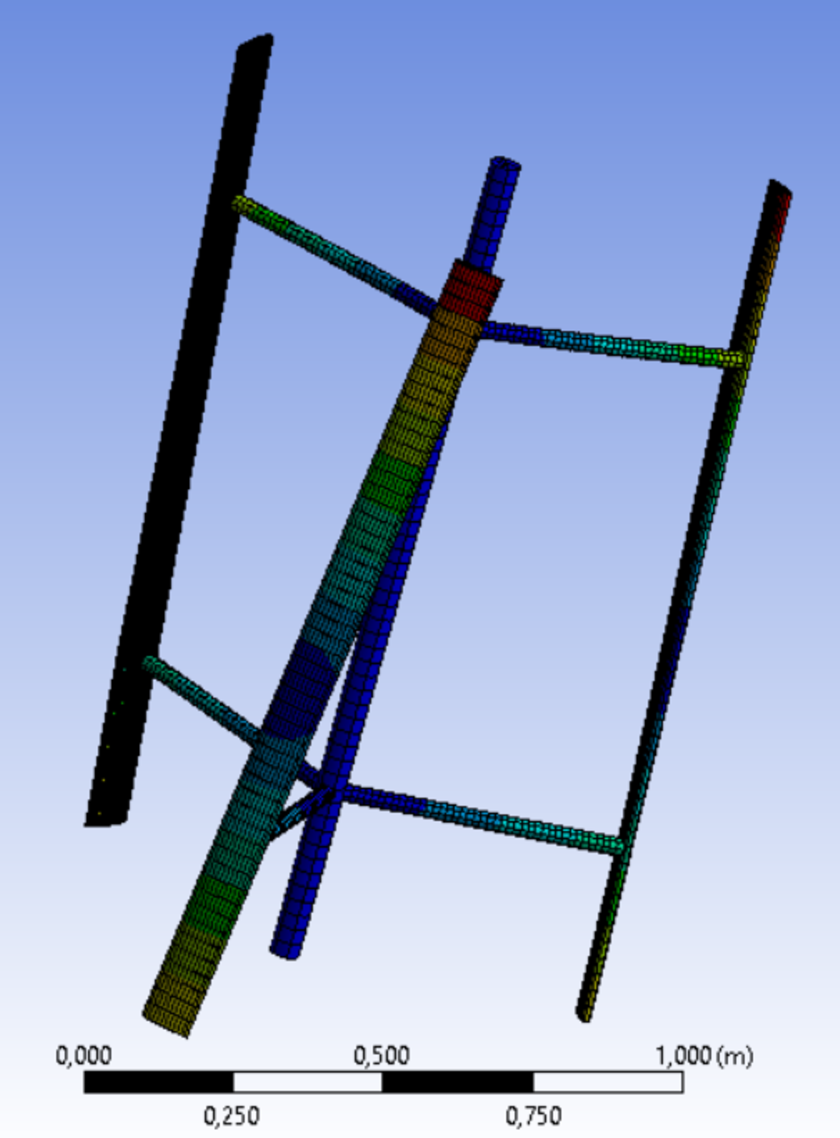
\includegraphics[width=0.95\textwidth]{figuras/resultmodalmacico6.pdf}
		\caption{Sexto modo.}
		\label{subfig:resultmodomacicomodo6}
	\end{subfigure}		
	\fonte{Autoria própria.}
\end{figure}


\section{Double-multiple streamtube model}
\label{sec:resultdmsm}

Em termos de torque, a \autoref{fig:resultCtPaFrontPost} apresenta o gráfico da coeficiente de torque para uma pá, onde é possível verificar que uma maior quantidade de torque é extraído no primeiro meio ciclo (0 - 180 graus) quando comparado com o segundo (180 - 360 graus).

\begin{figure}
	\centering
	\caption{Coeficiente de torque para uma pá.}
	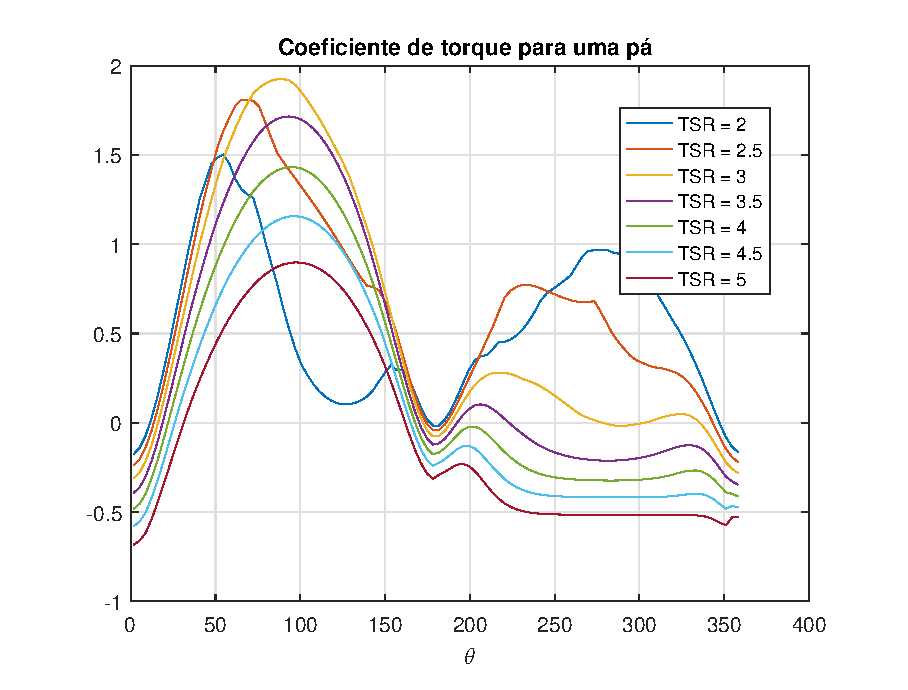
\includegraphics[width=0.8\textwidth]{figuras/resultCtPaFrontPost.eps}
	\fonte{Autoria própria.}
	\label{fig:resultCtPaFrontPost}
\end{figure}

\section{Próximas etapas}
\label{sec:trabalhosFuturos}

Os próximos passos a serem feitos estão sintetizados na \autoref{tab:cronograma}.

\begin{table}[H]
	\centering
	\caption{Cronograma.}
	\label{tab:cronograma}
	    \begin{tabular}{l c c c c c c}
        \hline TAREFA & SEM 1 & SEM 2 & SEM 3 & SEM 4 & SEM 5 & SEM 6\\
        \hline        
		Verificação da influencia da água & X & & & & & \\
		Acoplamento trem de potência & X & X & X & & & \\
		Elaboração e submissão de artigo & & & X & X & X &\\
		Redação final & X& X& X& X & X & X\\
		Submissão de versão final & & & & & & X \\
		\hline
    \end{tabular}

	\fonte{Autoria Própria.}
\end{table}

\begin{quadro}[!htb]
	\centering
	\caption{Exemplo de Quadro.\label{qua:quadro-exemplo1}}
	\begin{tabular}{|p{7cm}|p{7cm}|}
		\hline
		\textbf{BD Relacionais} & \textbf{BD Orientados a Objetos} \\
		\hline
		Os dados são passivos, ou seja, certas operações limitadas podem ser automaticamente acionadas quando os dados são usados. Os dados são ativos, ou seja, as solicitações fazem com que os objetos executem seus métodos. & Os processos que usam dados mudam constantemente. \\
		\hline
	\end{tabular}
	\fonte{XXXXXXXXXXXX.}
\end{quadro}